\subsection{\mHi=115 \GeV\ Analysis}

%%%%%%%%%%%%%%%%%%%%
\begin{figure}[!hbtp]
\centering
\subfigure[]{
\centering
\label{subfig:dPhi_mh115_nj0}
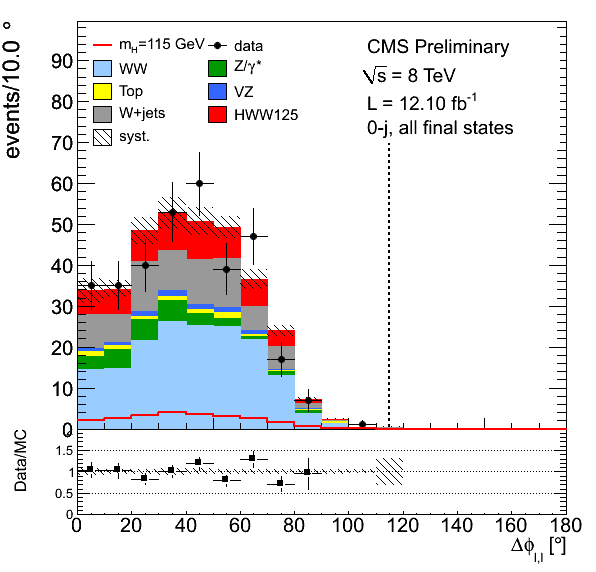
\includegraphics[width=.3\textwidth]{figures/dPhi_mh115_nj0.png}
}
\subfigure[]{
\centering
\label{subfig:dilepmass_mh115_nj0}
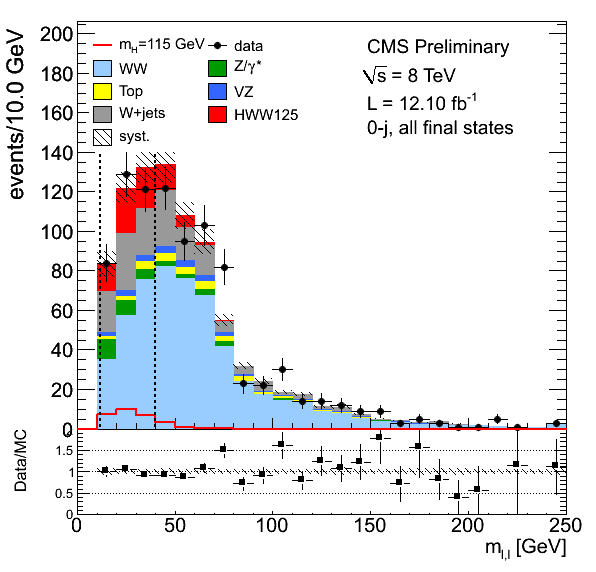
\includegraphics[width=.3\textwidth]{figures/dilepmass_mh115_nj0.png}
}
\\
\subfigure[]{
\centering
\label{subfig:dileppt_mh115_nj0}
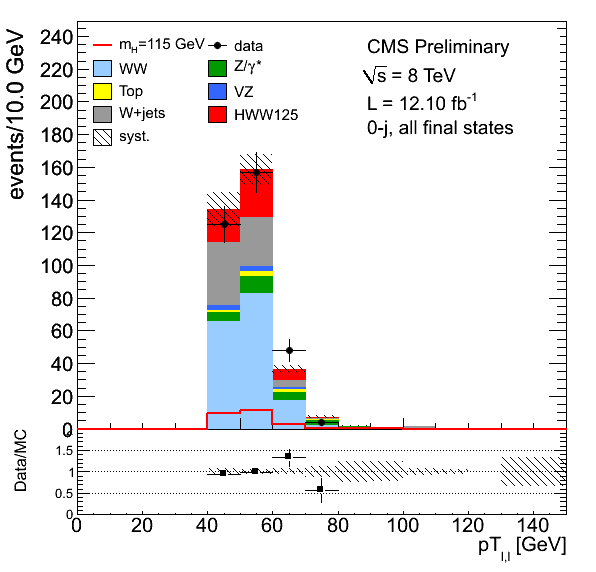
\includegraphics[width=.3\textwidth]{figures/dileppt_mh115_nj0.png}
}
\subfigure[]{
\centering
\label{subfig:jet1pt_mh115_nj0}
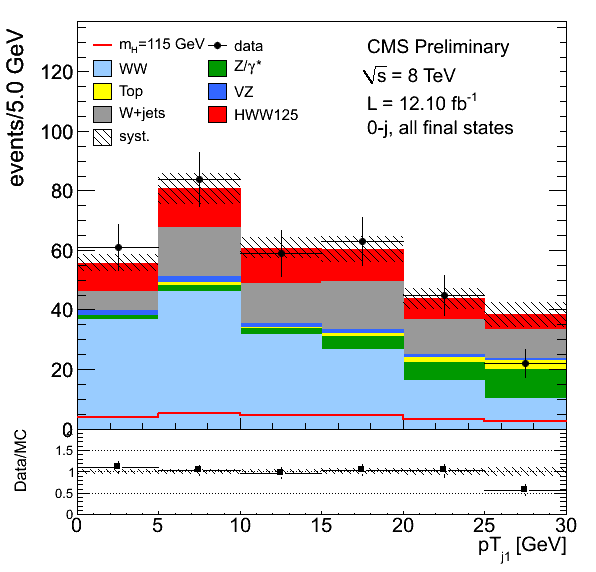
\includegraphics[width=.3\textwidth]{figures/jet1pt_mh115_nj0.png}
}
\\
\subfigure[]{
\centering
\label{subfig:lep1pt_mh115_nj0}
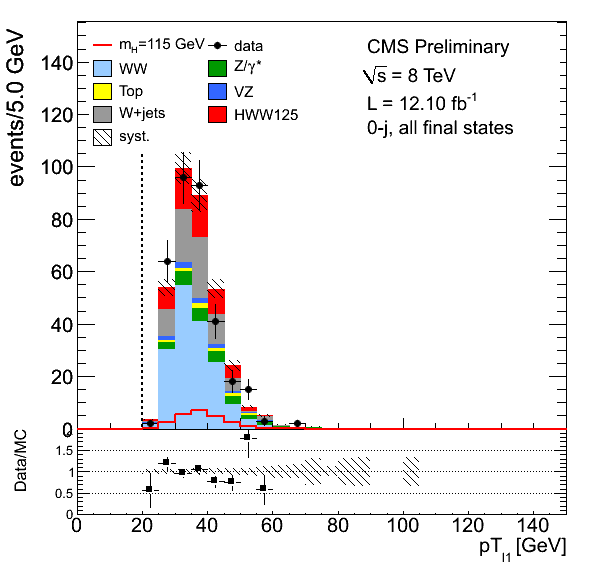
\includegraphics[width=.3\textwidth]{figures/lep1pt_mh115_nj0.png}
}
\subfigure[]{
\centering
\label{subfig:lep2pt_mh115_nj0}
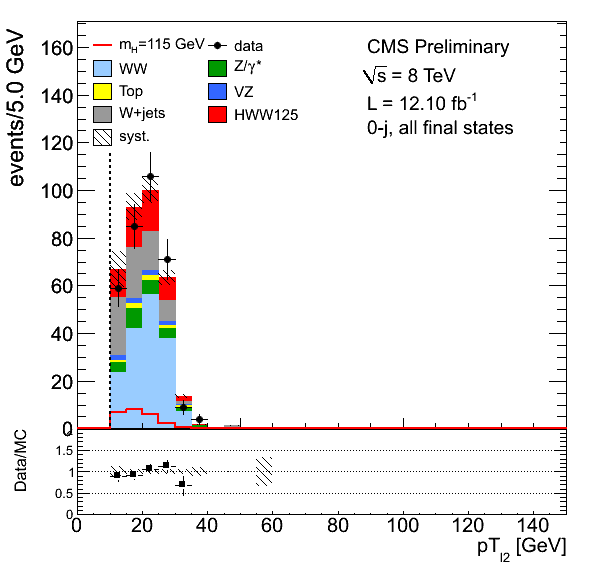
\includegraphics[width=.3\textwidth]{figures/lep2pt_mh115_nj0.png}
}
\\
\subfigure[]{
\centering
\label{subfig:mt_mh115_nj0}
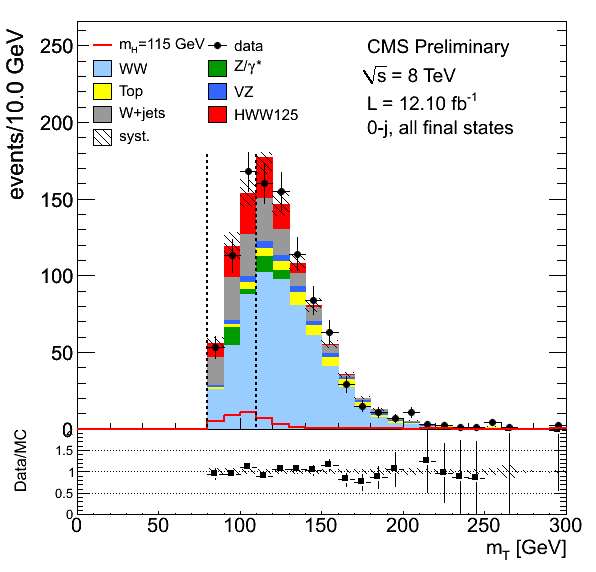
\includegraphics[width=.3\textwidth]{figures/mt_mh115_nj0.png}
}
\subfigure[]{
\centering
\label{subfig:type_mh115_nj0}
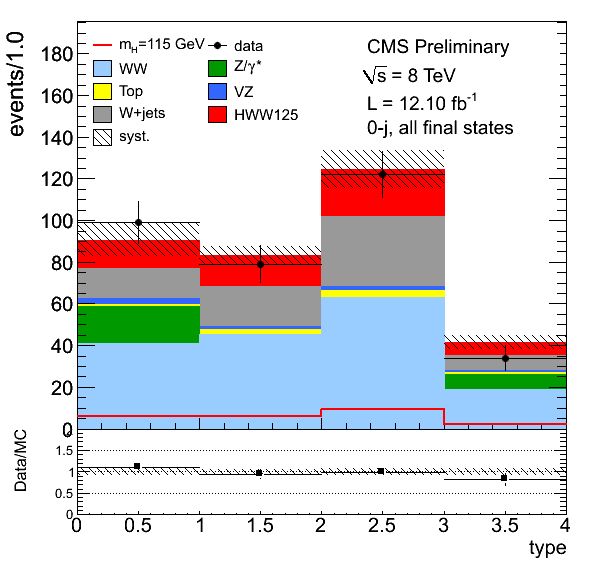
\includegraphics[width=.3\textwidth]{figures/type_mh115_nj0.png}
}
\\
\caption{Cut based analysis \mHi=115 \GeV, 0-jet bin.}
\label{fig:cutmh115_0j}
\end{figure}
%%%%%%%%%%%%%%%%%%%%

%%%%%%%%%%%%%%%%%%%%
\begin{figure}[!hbtp]
\centering
\subfigure[]{
\centering
\label{subfig:dPhi_mh115_nj1}
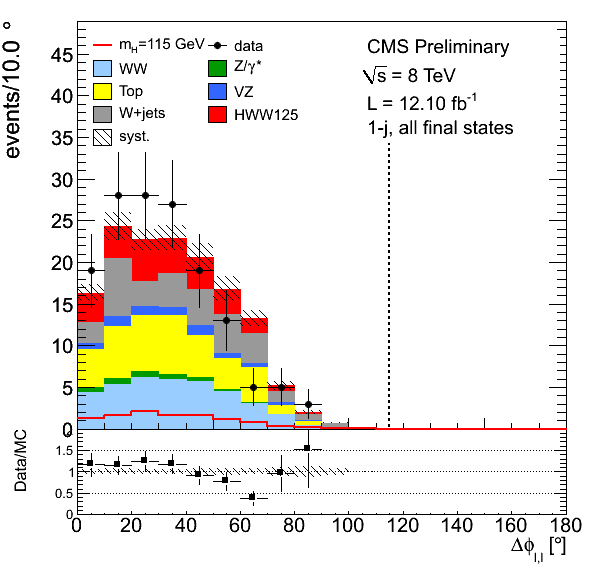
\includegraphics[width=.3\textwidth]{figures/dPhi_mh115_nj1.png}
}
\subfigure[]{
\centering
\label{subfig:dilepmass_mh115_nj1}
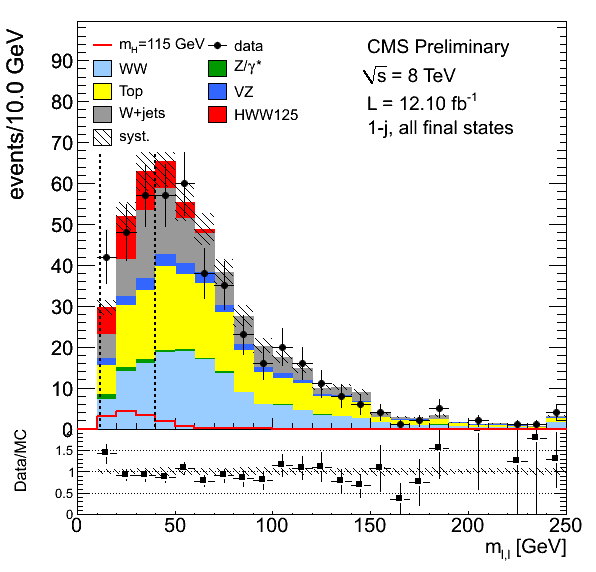
\includegraphics[width=.3\textwidth]{figures/dilepmass_mh115_nj1.png}
}
\\
\subfigure[]{
\centering
\label{subfig:dileppt_mh115_nj1}
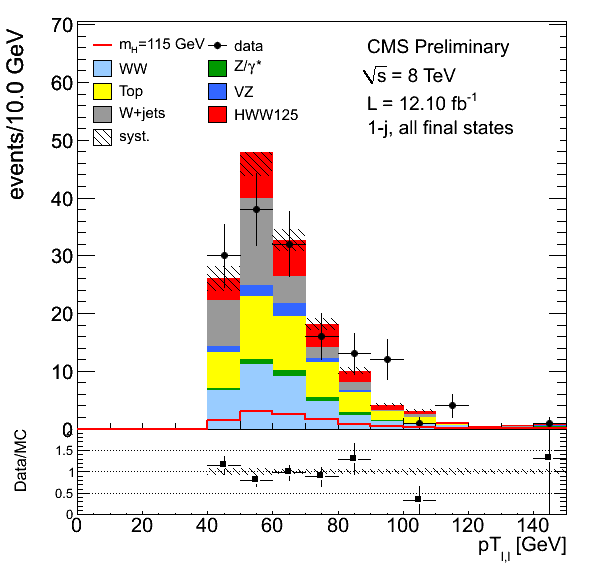
\includegraphics[width=.3\textwidth]{figures/dileppt_mh115_nj1.png}
}
\subfigure[]{
\centering
\label{subfig:jet1pt_mh115_nj1}
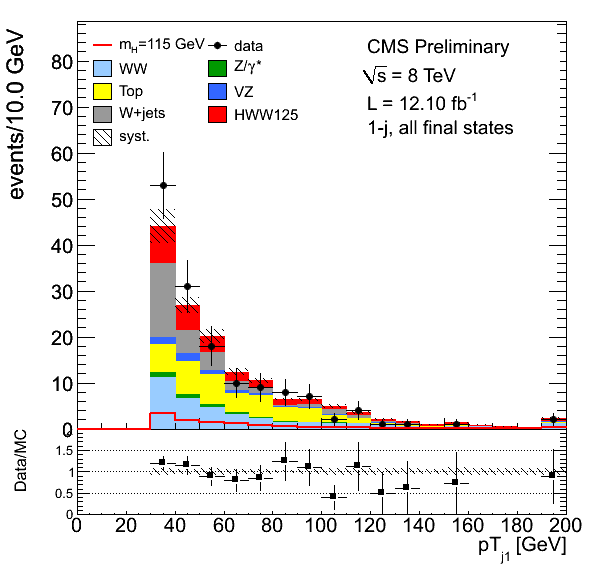
\includegraphics[width=.3\textwidth]{figures/jet1pt_mh115_nj1.png}
}
\\
\subfigure[]{
\centering
\label{subfig:lep1pt_mh115_nj1}
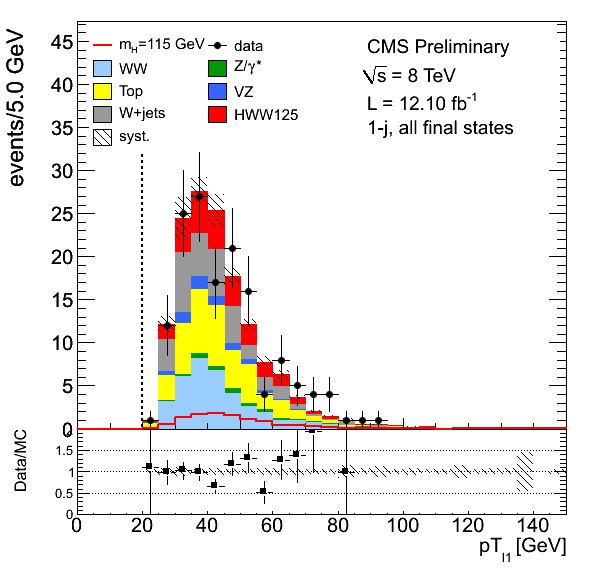
\includegraphics[width=.3\textwidth]{figures/lep1pt_mh115_nj1.png}
}
\subfigure[]{
\centering
\label{subfig:lep2pt_mh115_nj1}
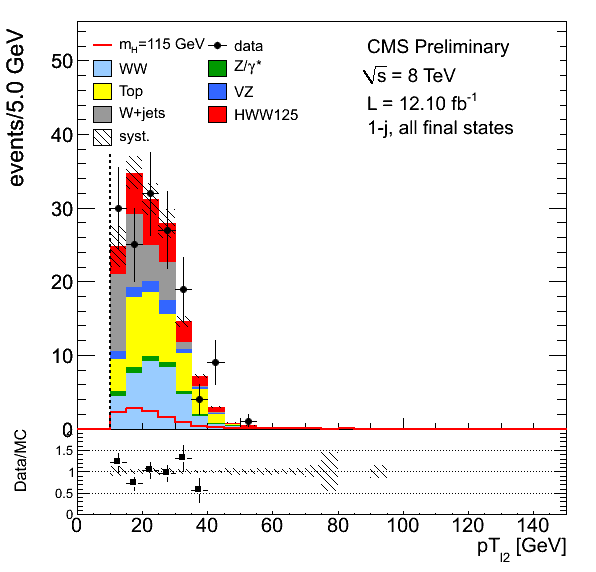
\includegraphics[width=.3\textwidth]{figures/lep2pt_mh115_nj1.png}
}
\\
\subfigure[]{
\centering
\label{subfig:mt_mh115_nj1}
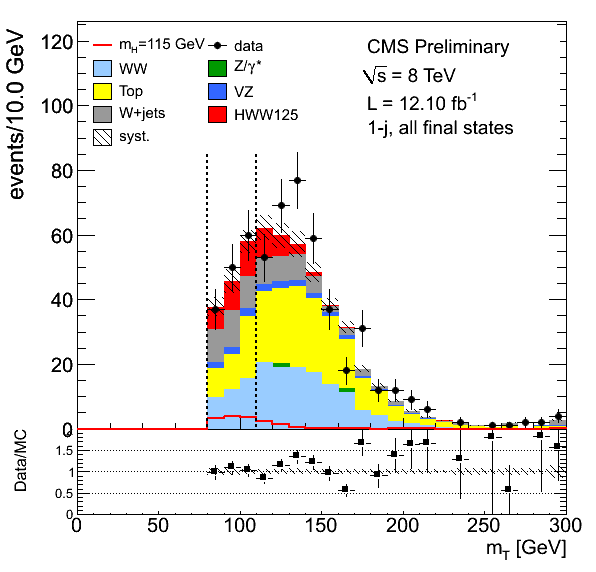
\includegraphics[width=.3\textwidth]{figures/mt_mh115_nj1.png}
}
\subfigure[]{
\centering
\label{subfig:type_mh115_nj1}
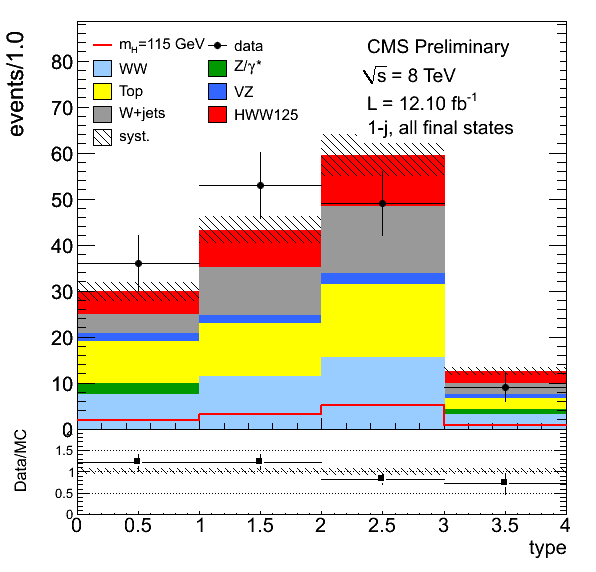
\includegraphics[width=.3\textwidth]{figures/type_mh115_nj1.png}
}
\\
\caption{Cut based analysis \mHi=115 \GeV, 1-jet bin.}
\label{fig:cutmh115_1j}
\end{figure}
%%%%%%%%%%%%%%%%%%%%

%%%%%%%%%%%%%%%%%%%%
\begin{figure}[!hbtp]
\centering
\subfigure[]{
\centering
\label{subfig:dPhi_mh115_nj2}
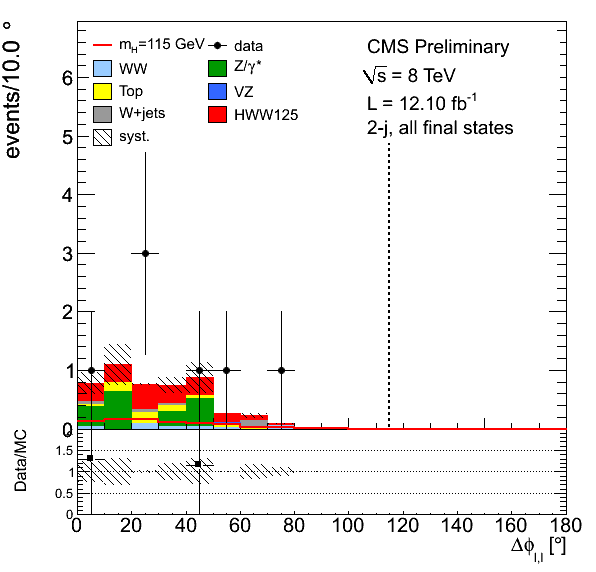
\includegraphics[width=.3\textwidth]{figures/dPhi_mh115_nj2.png}
}
\subfigure[]{
\centering
\label{subfig:dilepmass_mh115_nj2}
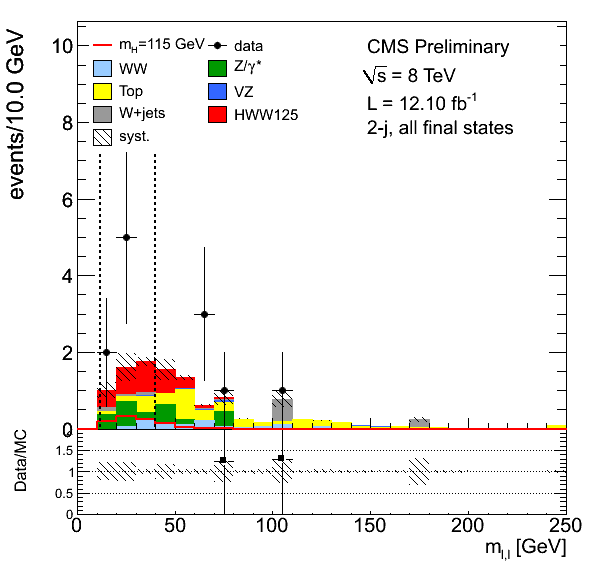
\includegraphics[width=.3\textwidth]{figures/dilepmass_mh115_nj2.png}
}
\\
\subfigure[]{
\centering
\label{subfig:dileppt_mh115_nj2}
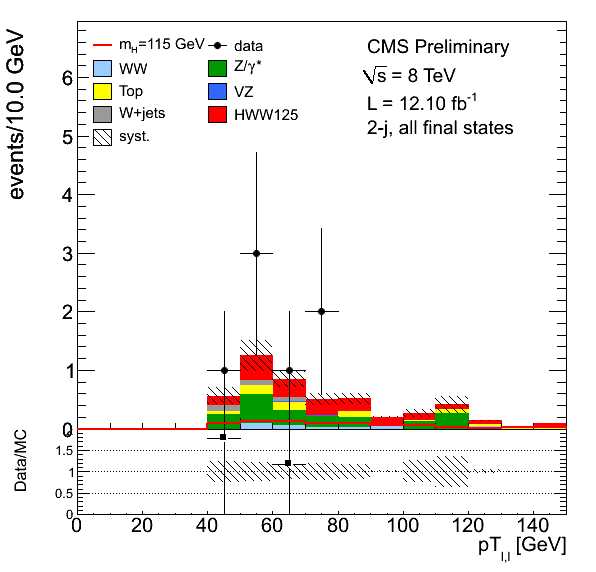
\includegraphics[width=.3\textwidth]{figures/dileppt_mh115_nj2.png}
}
\subfigure[]{
\centering
\label{subfig:jet1pt_mh115_nj2}
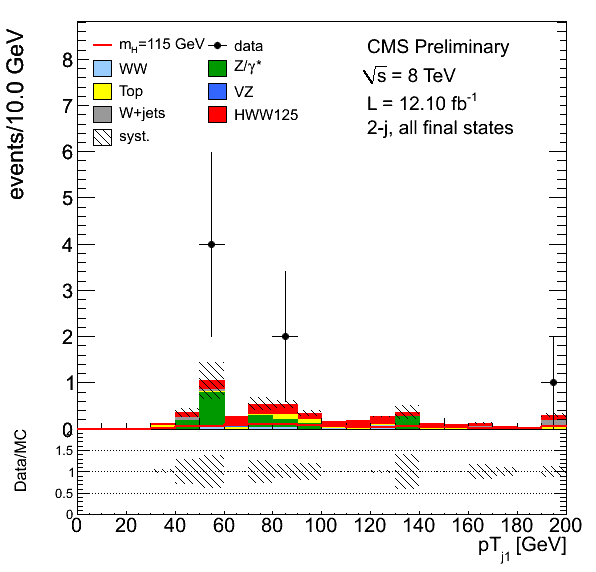
\includegraphics[width=.3\textwidth]{figures/jet1pt_mh115_nj2.png}
}
\\
\subfigure[]{
\centering
\label{subfig:lep1pt_mh115_nj2}
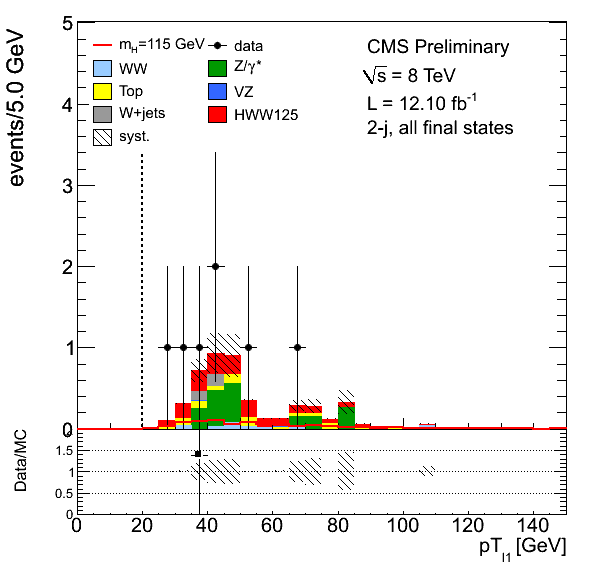
\includegraphics[width=.3\textwidth]{figures/lep1pt_mh115_nj2.png}
}
\subfigure[]{
\centering
\label{subfig:lep2pt_mh115_nj2}
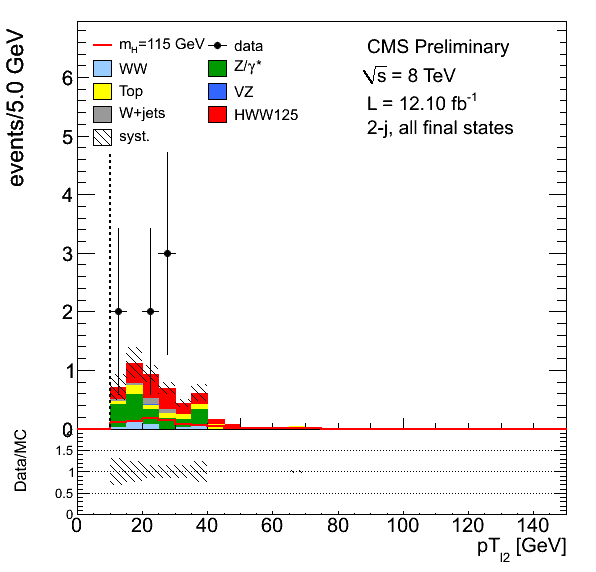
\includegraphics[width=.3\textwidth]{figures/lep2pt_mh115_nj2.png}
}
\\
\subfigure[]{
\centering
\label{subfig:mt_mh115_nj2}
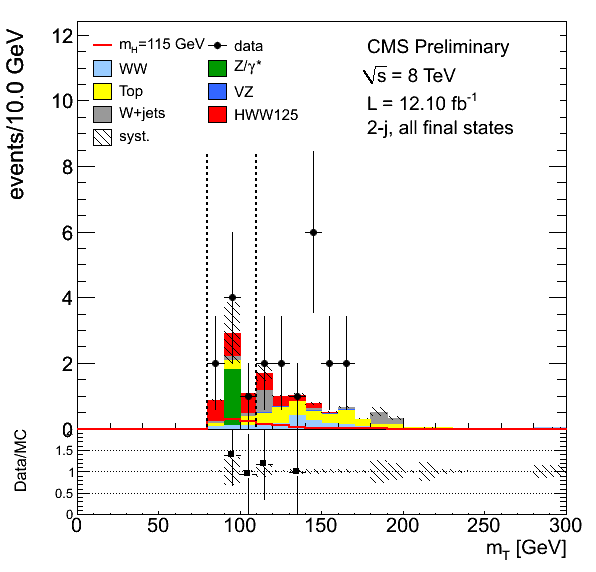
\includegraphics[width=.3\textwidth]{figures/mt_mh115_nj2.png}
}
\subfigure[]{
\centering
\label{subfig:type_mh115_nj2}
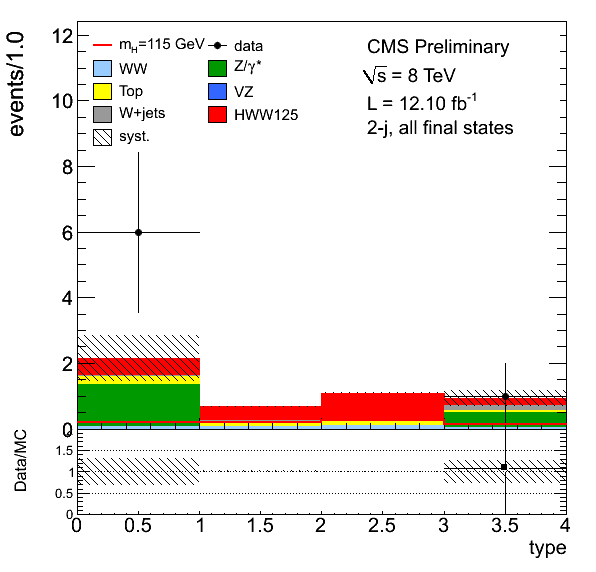
\includegraphics[width=.3\textwidth]{figures/type_mh115_nj2.png}
}
\\
\caption{Cut based analysis \mHi=115 \GeV, 2-jet bin.}
\label{fig:cutmh115_2j}
\end{figure}
%%%%%%%%%%%%%%%%%%%%


\subsection{\mHi=125 \GeV\ Analysis}

%%%%%%%%%%%%%%%%%%%%
\begin{figure}[!hbtp]
\centering
\subfigure[]{
\centering
\label{subfig:dPhi_mh125_nj0}
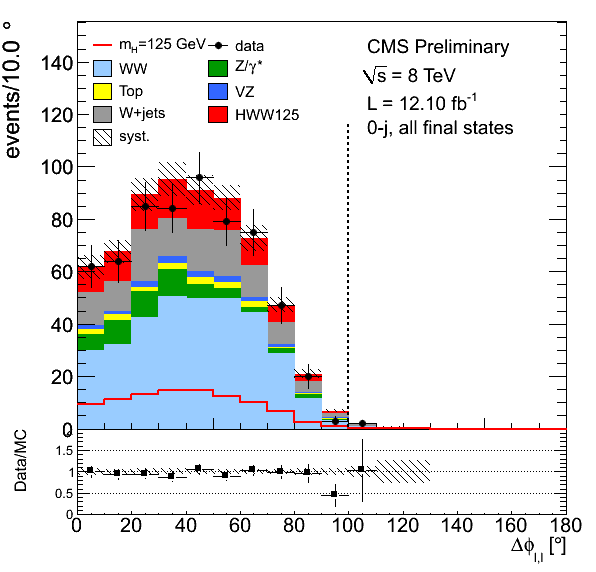
\includegraphics[width=.3\textwidth]{figures/dPhi_mh125_nj0.png}
}
\subfigure[]{
\centering
\label{subfig:dilepmass_mh125_nj0}
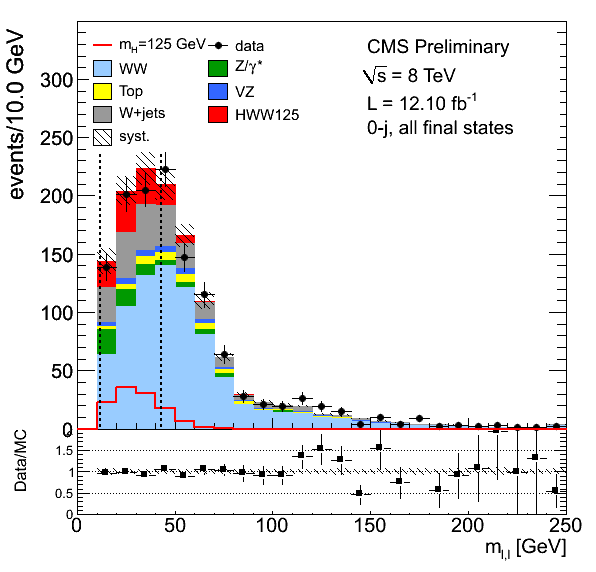
\includegraphics[width=.3\textwidth]{figures/dilepmass_mh125_nj0.png}
}
\\
\subfigure[]{
\centering
\label{subfig:dileppt_mh125_nj0}
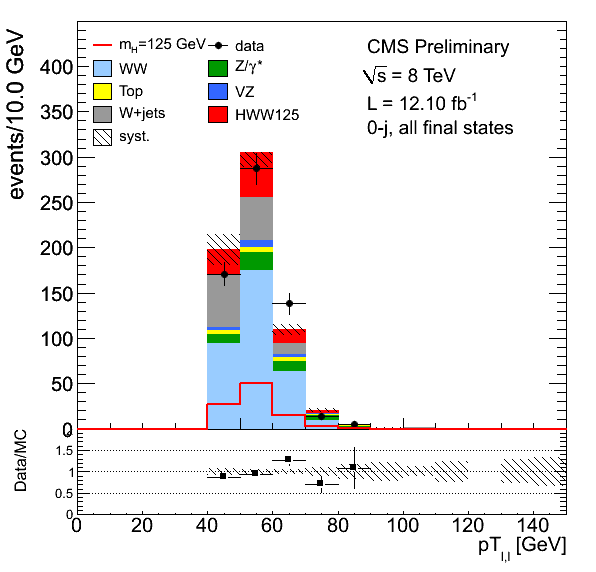
\includegraphics[width=.3\textwidth]{figures/dileppt_mh125_nj0.png}
}
\subfigure[]{
\centering
\label{subfig:jet1pt_mh125_nj0}
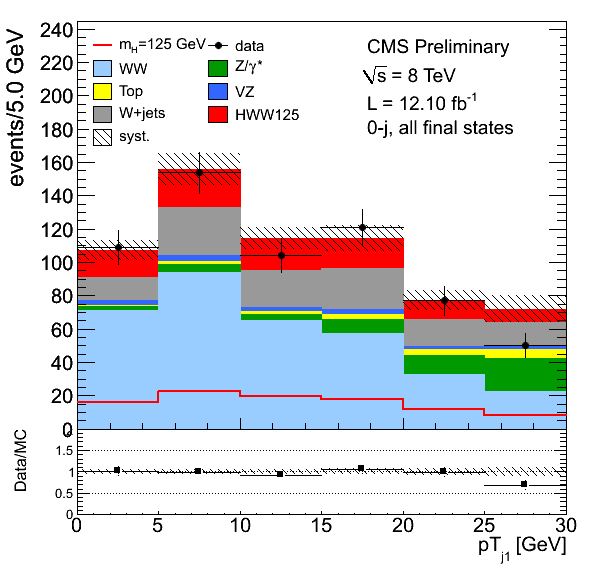
\includegraphics[width=.3\textwidth]{figures/jet1pt_mh125_nj0.png}
}
\\
\subfigure[]{
\centering
\label{subfig:lep1pt_mh125_nj0}
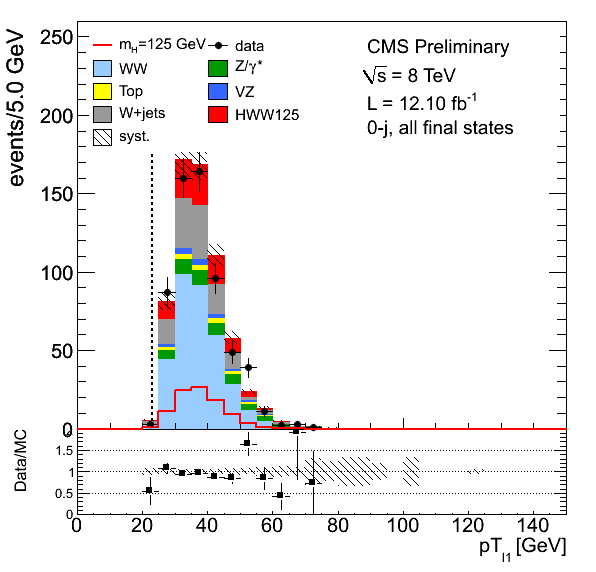
\includegraphics[width=.3\textwidth]{figures/lep1pt_mh125_nj0.png}
}
\subfigure[]{
\centering
\label{subfig:lep2pt_mh125_nj0}
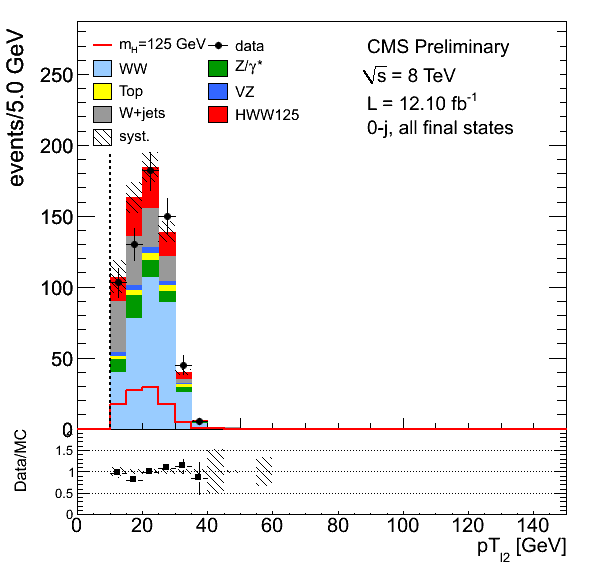
\includegraphics[width=.3\textwidth]{figures/lep2pt_mh125_nj0.png}
}
\\
\subfigure[]{
\centering
\label{subfig:mt_mh125_nj0}
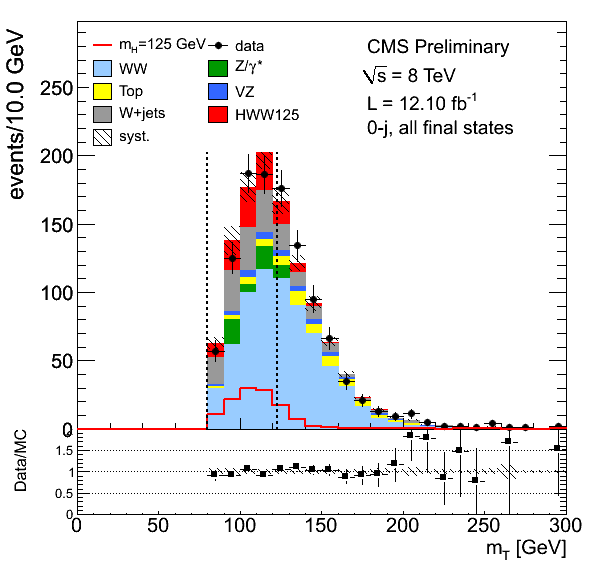
\includegraphics[width=.3\textwidth]{figures/mt_mh125_nj0.png}
}
\subfigure[]{
\centering
\label{subfig:type_mh125_nj0}
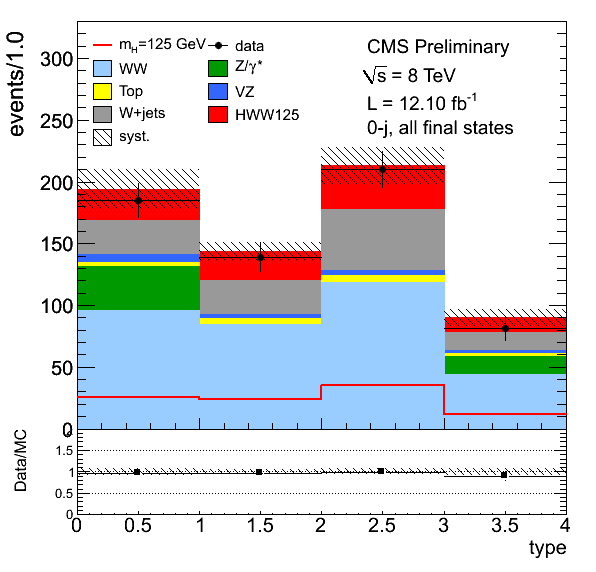
\includegraphics[width=.3\textwidth]{figures/type_mh125_nj0.png}
}
\\
\caption{Cut based analysis \mHi=125 \GeV, 0-jet bin.}
\label{fig:cutmh125_0j}
\end{figure}
%%%%%%%%%%%%%%%%%%%%

%%%%%%%%%%%%%%%%%%%%
\begin{figure}[!hbtp]
\centering
\subfigure[]{
\centering
\label{subfig:dPhi_mh125_nj1}
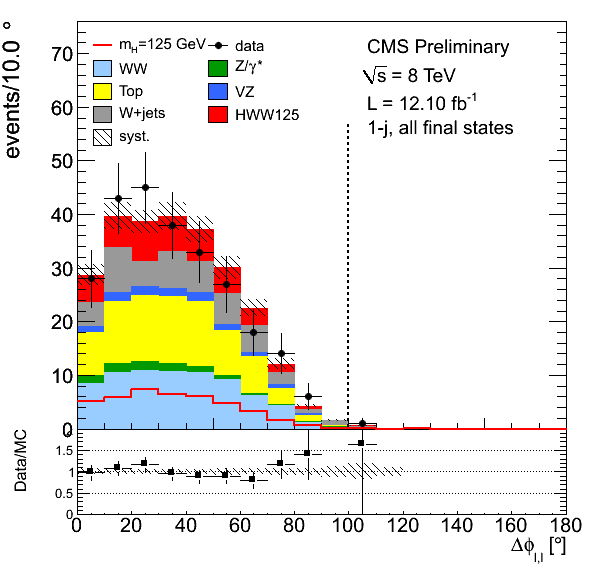
\includegraphics[width=.3\textwidth]{figures/dPhi_mh125_nj1.png}
}
\subfigure[]{
\centering
\label{subfig:dilepmass_mh125_nj1}
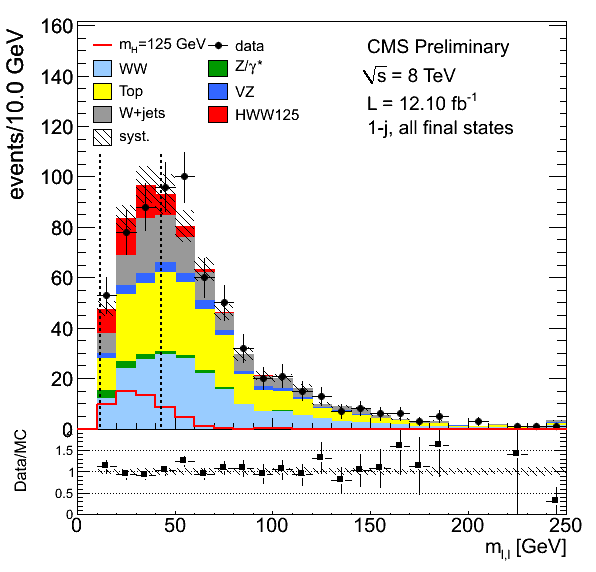
\includegraphics[width=.3\textwidth]{figures/dilepmass_mh125_nj1.png}
}
\\
\subfigure[]{
\centering
\label{subfig:dileppt_mh125_nj1}
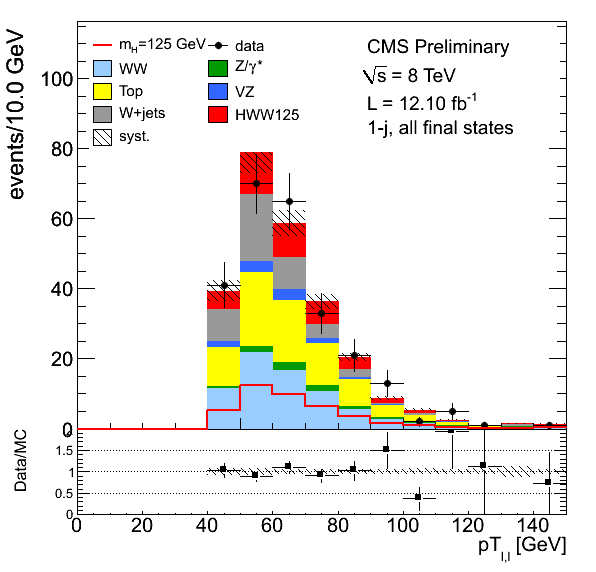
\includegraphics[width=.3\textwidth]{figures/dileppt_mh125_nj1.png}
}
\subfigure[]{
\centering
\label{subfig:jet1pt_mh125_nj1}
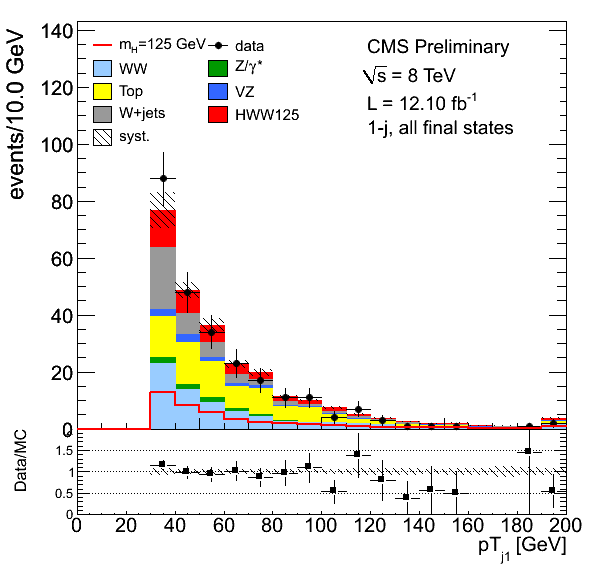
\includegraphics[width=.3\textwidth]{figures/jet1pt_mh125_nj1.png}
}
\\
\subfigure[]{
\centering
\label{subfig:lep1pt_mh125_nj1}
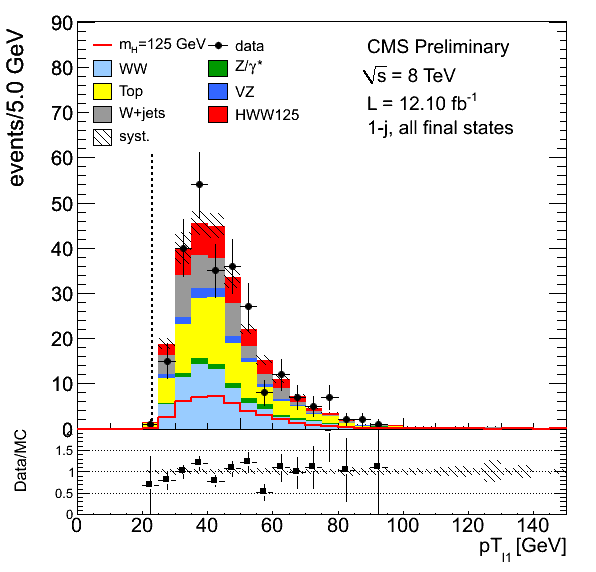
\includegraphics[width=.3\textwidth]{figures/lep1pt_mh125_nj1.png}
}
\subfigure[]{
\centering
\label{subfig:lep2pt_mh125_nj1}
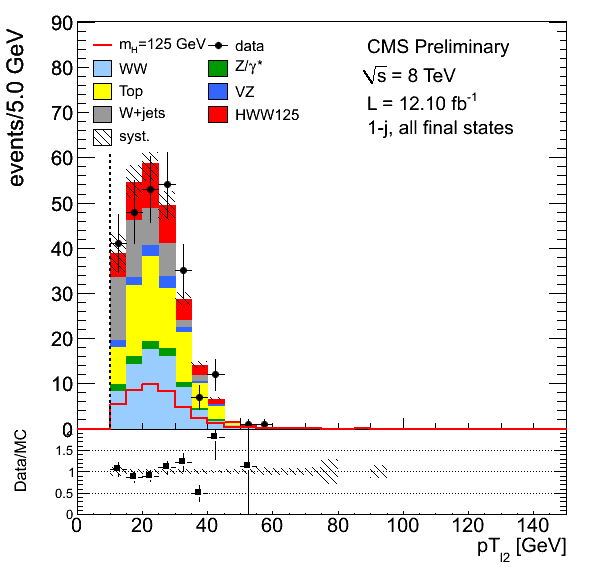
\includegraphics[width=.3\textwidth]{figures/lep2pt_mh125_nj1.png}
}
\\
\subfigure[]{
\centering
\label{subfig:mt_mh125_nj1}
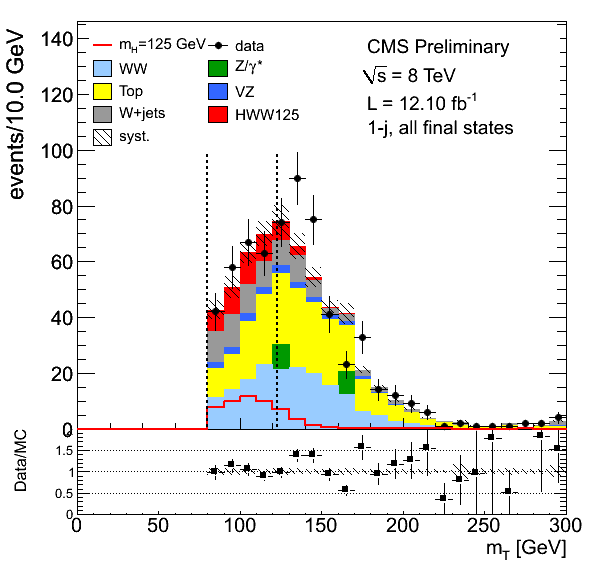
\includegraphics[width=.3\textwidth]{figures/mt_mh125_nj1.png}
}
\subfigure[]{
\centering
\label{subfig:type_mh125_nj1}
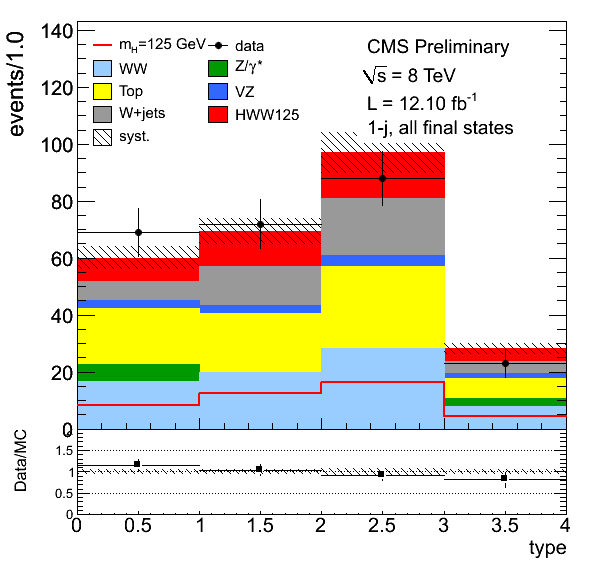
\includegraphics[width=.3\textwidth]{figures/type_mh125_nj1.png}
}
\\
\caption{Cut based analysis \mHi=125 \GeV, 1-jet bin.}
\label{fig:cutmh125_1j}
\end{figure}
%%%%%%%%%%%%%%%%%%%%

%%%%%%%%%%%%%%%%%%%%
\begin{figure}[!hbtp]
\centering
\subfigure[]{
\centering
\label{subfig:dPhi_mh125_nj2}
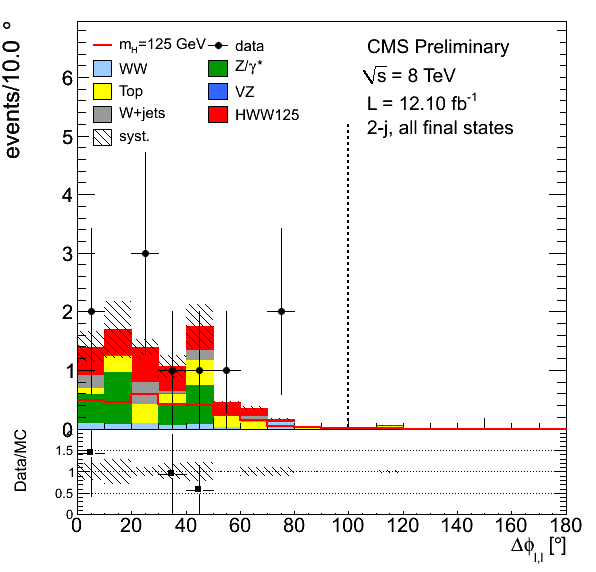
\includegraphics[width=.3\textwidth]{figures/dPhi_mh125_nj2.png}
}
\subfigure[]{
\centering
\label{subfig:dilepmass_mh125_nj2}
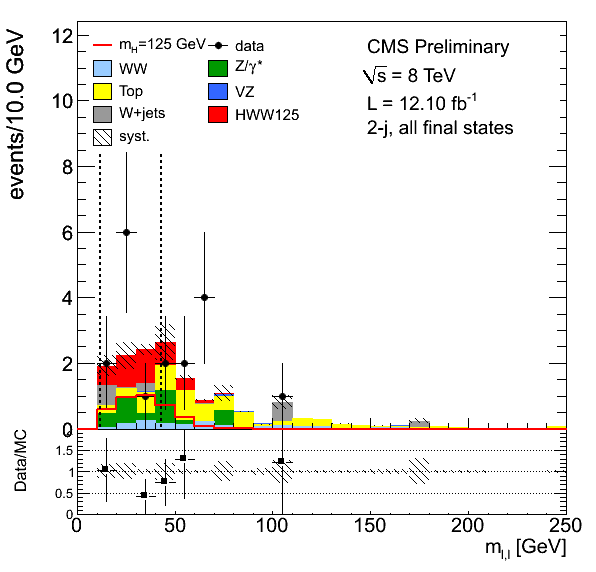
\includegraphics[width=.3\textwidth]{figures/dilepmass_mh125_nj2.png}
}
\\
\subfigure[]{
\centering
\label{subfig:dileppt_mh125_nj2}
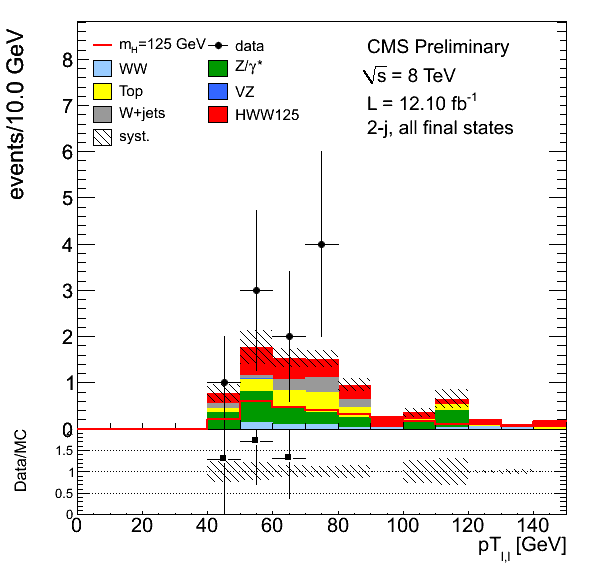
\includegraphics[width=.3\textwidth]{figures/dileppt_mh125_nj2.png}
}
\subfigure[]{
\centering
\label{subfig:jet1pt_mh125_nj2}
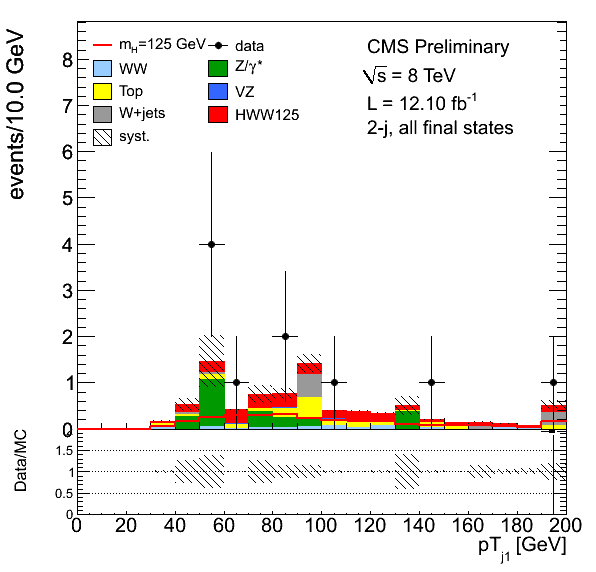
\includegraphics[width=.3\textwidth]{figures/jet1pt_mh125_nj2.png}
}
\\
\subfigure[]{
\centering
\label{subfig:lep1pt_mh125_nj2}
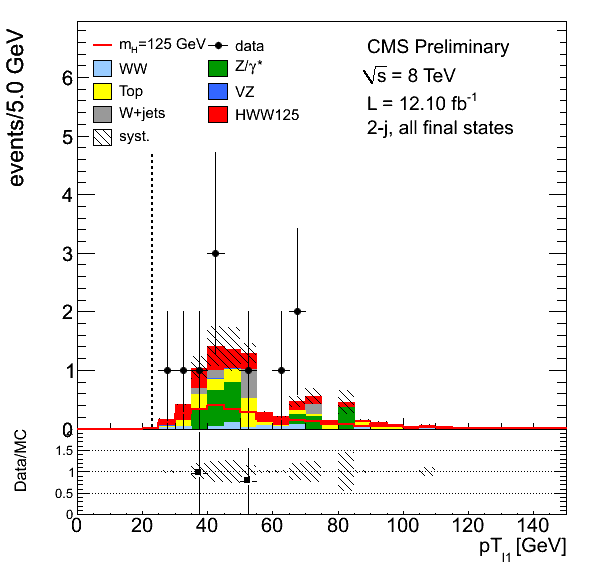
\includegraphics[width=.3\textwidth]{figures/lep1pt_mh125_nj2.png}
}
\subfigure[]{
\centering
\label{subfig:lep2pt_mh125_nj2}
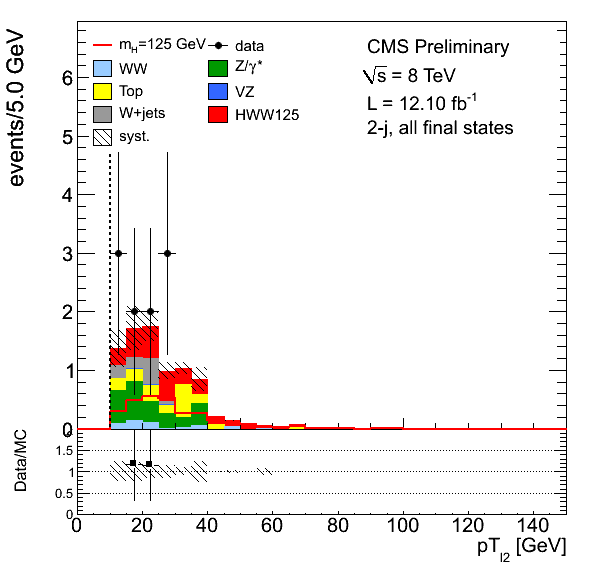
\includegraphics[width=.3\textwidth]{figures/lep2pt_mh125_nj2.png}
}
\\
\subfigure[]{
\centering
\label{subfig:mt_mh125_nj2}
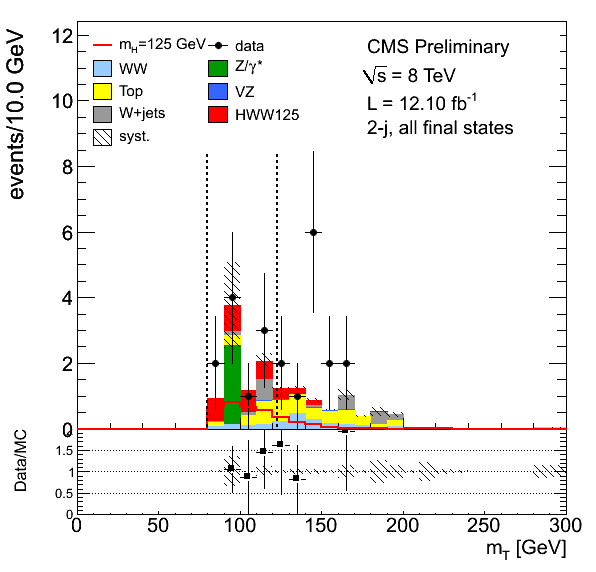
\includegraphics[width=.3\textwidth]{figures/mt_mh125_nj2.png}
}
\subfigure[]{
\centering
\label{subfig:type_mh125_nj2}
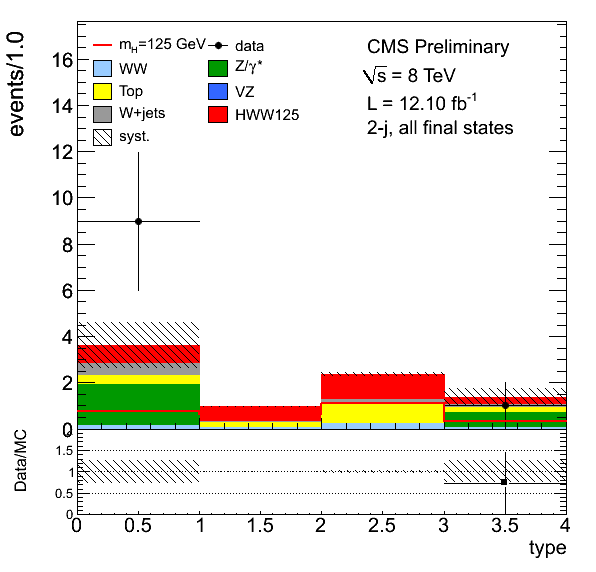
\includegraphics[width=.3\textwidth]{figures/type_mh125_nj2.png}
}
\\
\caption{Cut based analysis \mHi=125 \GeV, 2-jet bin.}
\label{fig:cutmh125_2j}
\end{figure}
%%%%%%%%%%%%%%%%%%%%


\subsection{\mHi=140 \GeV\ Analysis}

%%%%%%%%%%%%%%%%%%%%
\begin{figure}[!hbtp]
\centering
\subfigure[]{
\centering
\label{subfig:dPhi_mh140_nj0}
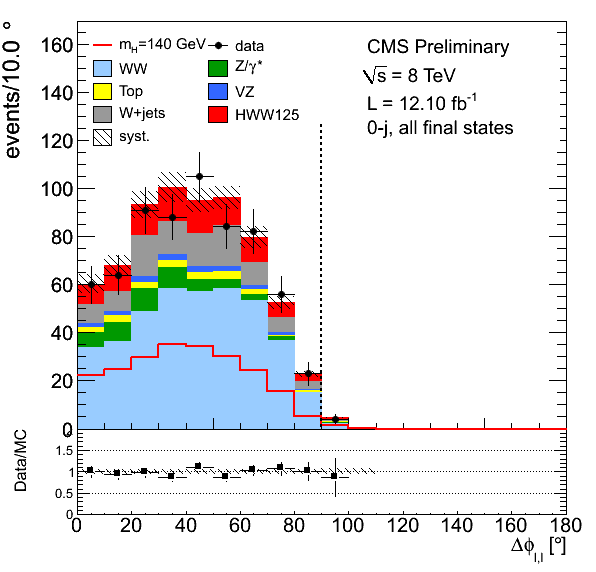
\includegraphics[width=.3\textwidth]{figures/dPhi_mh140_nj0.png}
}
\subfigure[]{
\centering
\label{subfig:dilepmass_mh140_nj0}
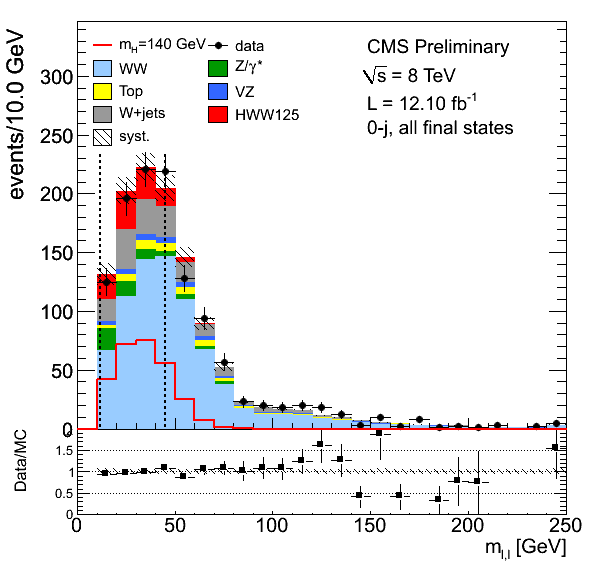
\includegraphics[width=.3\textwidth]{figures/dilepmass_mh140_nj0.png}
}
\\
\subfigure[]{
\centering
\label{subfig:dileppt_mh140_nj0}
\includegraphics[width=.3\textwidth]{figures/dileppt_mh140_nj0.png}
}
\subfigure[]{
\centering
\label{subfig:jet1pt_mh140_nj0}
\includegraphics[width=.3\textwidth]{figures/jet1pt_mh140_nj0.png}
}
\\
\subfigure[]{
\centering
\label{subfig:lep1pt_mh140_nj0}
\includegraphics[width=.3\textwidth]{figures/lep1pt_mh140_nj0.png}
}
\subfigure[]{
\centering
\label{subfig:lep2pt_mh140_nj0}
\includegraphics[width=.3\textwidth]{figures/lep2pt_mh140_nj0.png}
}
\\
\subfigure[]{
\centering
\label{subfig:mt_mh140_nj0}
\includegraphics[width=.3\textwidth]{figures/mt_mh140_nj0.png}
}
\subfigure[]{
\centering
\label{subfig:type_mh140_nj0}
\includegraphics[width=.3\textwidth]{figures/type_mh140_nj0.png}
}
\\
\caption{Cut based analysis \mHi=140 \GeV, 0-jet bin.}
\label{fig:cutmh140_0j}
\end{figure}
%%%%%%%%%%%%%%%%%%%%

%%%%%%%%%%%%%%%%%%%%
\begin{figure}[!hbtp]
\centering
\subfigure[]{
\centering
\label{subfig:dPhi_mh140_nj1}
\includegraphics[width=.3\textwidth]{figures/dPhi_mh140_nj1.png}
}
\subfigure[]{
\centering
\label{subfig:dilepmass_mh140_nj1}
\includegraphics[width=.3\textwidth]{figures/dilepmass_mh140_nj1.png}
}
\\
\subfigure[]{
\centering
\label{subfig:dileppt_mh140_nj1}
\includegraphics[width=.3\textwidth]{figures/dileppt_mh140_nj1.png}
}
\subfigure[]{
\centering
\label{subfig:jet1pt_mh140_nj1}
\includegraphics[width=.3\textwidth]{figures/jet1pt_mh140_nj1.png}
}
\\
\subfigure[]{
\centering
\label{subfig:lep1pt_mh140_nj1}
\includegraphics[width=.3\textwidth]{figures/lep1pt_mh140_nj1.png}
}
\subfigure[]{
\centering
\label{subfig:lep2pt_mh140_nj1}
\includegraphics[width=.3\textwidth]{figures/lep2pt_mh140_nj1.png}
}
\\
\subfigure[]{
\centering
\label{subfig:mt_mh140_nj1}
\includegraphics[width=.3\textwidth]{figures/mt_mh140_nj1.png}
}
\subfigure[]{
\centering
\label{subfig:type_mh140_nj1}
\includegraphics[width=.3\textwidth]{figures/type_mh140_nj1.png}
}
\\
\caption{Cut based analysis \mHi=140 \GeV, 1-jet bin.}
\label{fig:cutmh140_1j}
\end{figure}
%%%%%%%%%%%%%%%%%%%%

%%%%%%%%%%%%%%%%%%%%
\begin{figure}[!hbtp]
\centering
\subfigure[]{
\centering
\label{subfig:dPhi_mh140_nj2}
\includegraphics[width=.3\textwidth]{figures/dPhi_mh140_nj2.png}
}
\subfigure[]{
\centering
\label{subfig:dilepmass_mh140_nj2}
\includegraphics[width=.3\textwidth]{figures/dilepmass_mh140_nj2.png}
}
\\
\subfigure[]{
\centering
\label{subfig:dileppt_mh140_nj2}
\includegraphics[width=.3\textwidth]{figures/dileppt_mh140_nj2.png}
}
\subfigure[]{
\centering
\label{subfig:jet1pt_mh140_nj2}
\includegraphics[width=.3\textwidth]{figures/jet1pt_mh140_nj2.png}
}
\\
\subfigure[]{
\centering
\label{subfig:lep1pt_mh140_nj2}
\includegraphics[width=.3\textwidth]{figures/lep1pt_mh140_nj2.png}
}
\subfigure[]{
\centering
\label{subfig:lep2pt_mh140_nj2}
\includegraphics[width=.3\textwidth]{figures/lep2pt_mh140_nj2.png}
}
\\
\subfigure[]{
\centering
\label{subfig:mt_mh140_nj2}
\includegraphics[width=.3\textwidth]{figures/mt_mh140_nj2.png}
}
\subfigure[]{
\centering
\label{subfig:type_mh140_nj2}
\includegraphics[width=.3\textwidth]{figures/type_mh140_nj2.png}
}
\\
\caption{Cut based analysis \mHi=140 \GeV, 2-jet bin.}
\label{fig:cutmh140_2j}
\end{figure}
%%%%%%%%%%%%%%%%%%%%



\subsection{\mHi=160 \GeV\ Analysis}

%%%%%%%%%%%%%%%%%%%%
\begin{figure}[!hbtp]
\centering
\subfigure[]{
\centering
\label{subfig:dPhi_mh160_nj0}
\includegraphics[width=.3\textwidth]{figures/dPhi_mh160_nj0.png}
}
\subfigure[]{
\centering
\label{subfig:dilepmass_mh160_nj0}
\includegraphics[width=.3\textwidth]{figures/dilepmass_mh160_nj0.png}
}
\\
\subfigure[]{
\centering
\label{subfig:dileppt_mh160_nj0}
\includegraphics[width=.3\textwidth]{figures/dileppt_mh160_nj0.png}
}
\subfigure[]{
\centering
\label{subfig:jet1pt_mh160_nj0}
\includegraphics[width=.3\textwidth]{figures/jet1pt_mh160_nj0.png}
}
\\
\subfigure[]{
\centering
\label{subfig:lep1pt_mh160_nj0}
\includegraphics[width=.3\textwidth]{figures/lep1pt_mh160_nj0.png}
}
\subfigure[]{
\centering
\label{subfig:lep2pt_mh160_nj0}
\includegraphics[width=.3\textwidth]{figures/lep2pt_mh160_nj0.png}
}
\\
\subfigure[]{
\centering
\label{subfig:mt_mh160_nj0}
\includegraphics[width=.3\textwidth]{figures/mt_mh160_nj0.png}
}
\subfigure[]{
\centering
\label{subfig:type_mh160_nj0}
\includegraphics[width=.3\textwidth]{figures/type_mh160_nj0.png}
}
\\
\caption{Cut based analysis \mHi=160 \GeV, 0-jet bin.}
\label{fig:cutmh160_0j}
\end{figure}
%%%%%%%%%%%%%%%%%%%%

%%%%%%%%%%%%%%%%%%%%
\begin{figure}[!hbtp]
\centering
\subfigure[]{
\centering
\label{subfig:dPhi_mh160_nj1}
\includegraphics[width=.3\textwidth]{figures/dPhi_mh160_nj1.png}
}
\subfigure[]{
\centering
\label{subfig:dilepmass_mh160_nj1}
\includegraphics[width=.3\textwidth]{figures/dilepmass_mh160_nj1.png}
}
\\
\subfigure[]{
\centering
\label{subfig:dileppt_mh160_nj1}
\includegraphics[width=.3\textwidth]{figures/dileppt_mh160_nj1.png}
}
\subfigure[]{
\centering
\label{subfig:jet1pt_mh160_nj1}
\includegraphics[width=.3\textwidth]{figures/jet1pt_mh160_nj1.png}
}
\\
\subfigure[]{
\centering
\label{subfig:lep1pt_mh160_nj1}
\includegraphics[width=.3\textwidth]{figures/lep1pt_mh160_nj1.png}
}
\subfigure[]{
\centering
\label{subfig:lep2pt_mh160_nj1}
\includegraphics[width=.3\textwidth]{figures/lep2pt_mh160_nj1.png}
}
\\
\subfigure[]{
\centering
\label{subfig:mt_mh160_nj1}
\includegraphics[width=.3\textwidth]{figures/mt_mh160_nj1.png}
}
\subfigure[]{
\centering
\label{subfig:type_mh160_nj1}
\includegraphics[width=.3\textwidth]{figures/type_mh160_nj1.png}
}
\\
\caption{Cut based analysis \mHi=160 \GeV, 1-jet bin.}
\label{fig:cutmh160_1j}
\end{figure}
%%%%%%%%%%%%%%%%%%%%

%%%%%%%%%%%%%%%%%%%%
\begin{figure}[!hbtp]
\centering
\subfigure[]{
\centering
\label{subfig:dPhi_mh160_nj2}
\includegraphics[width=.3\textwidth]{figures/dPhi_mh160_nj2.png}
}
\subfigure[]{
\centering
\label{subfig:dilepmass_mh160_nj2}
\includegraphics[width=.3\textwidth]{figures/dilepmass_mh160_nj2.png}
}
\\
\subfigure[]{
\centering
\label{subfig:dileppt_mh160_nj2}
\includegraphics[width=.3\textwidth]{figures/dileppt_mh160_nj2.png}
}
\subfigure[]{
\centering
\label{subfig:jet1pt_mh160_nj2}
\includegraphics[width=.3\textwidth]{figures/jet1pt_mh160_nj2.png}
}
\\
\subfigure[]{
\centering
\label{subfig:lep1pt_mh160_nj2}
\includegraphics[width=.3\textwidth]{figures/lep1pt_mh160_nj2.png}
}
\subfigure[]{
\centering
\label{subfig:lep2pt_mh160_nj2}
\includegraphics[width=.3\textwidth]{figures/lep2pt_mh160_nj2.png}
}
\\
\subfigure[]{
\centering
\label{subfig:mt_mh160_nj2}
\includegraphics[width=.3\textwidth]{figures/mt_mh160_nj2.png}
}
\subfigure[]{
\centering
\label{subfig:type_mh160_nj2}
\includegraphics[width=.3\textwidth]{figures/type_mh160_nj2.png}
}
\\
\caption{Cut based analysis \mHi=160 \GeV, 2-jet bin.}
\label{fig:cutmh160_2j}
\end{figure}
%%%%%%%%%%%%%%%%%%%%



\subsection{\mHi=200 \GeV\ Analysis}

%%%%%%%%%%%%%%%%%%%%
\begin{figure}[!hbtp]
\centering
\subfigure[]{
\centering
\label{subfig:dPhi_mh200_nj0}
\includegraphics[width=.3\textwidth]{figures/dPhi_mh200_nj0.png}
}
\subfigure[]{
\centering
\label{subfig:dilepmass_mh200_nj0}
\includegraphics[width=.3\textwidth]{figures/dilepmass_mh200_nj0.png}
}
\\
\subfigure[]{
\centering
\label{subfig:dileppt_mh200_nj0}
\includegraphics[width=.3\textwidth]{figures/dileppt_mh200_nj0.png}
}
\subfigure[]{
\centering
\label{subfig:jet1pt_mh200_nj0}
\includegraphics[width=.3\textwidth]{figures/jet1pt_mh200_nj0.png}
}
\\
\subfigure[]{
\centering
\label{subfig:lep1pt_mh200_nj0}
\includegraphics[width=.3\textwidth]{figures/lep1pt_mh200_nj0.png}
}
\subfigure[]{
\centering
\label{subfig:lep2pt_mh200_nj0}
\includegraphics[width=.3\textwidth]{figures/lep2pt_mh200_nj0.png}
}
\\
\subfigure[]{
\centering
\label{subfig:mt_mh200_nj0}
\includegraphics[width=.3\textwidth]{figures/mt_mh200_nj0.png}
}
\subfigure[]{
\centering
\label{subfig:type_mh200_nj0}
\includegraphics[width=.3\textwidth]{figures/type_mh200_nj0.png}
}
\\
\caption{Cut based analysis \mHi=200 \GeV, 0-jet bin.}
\label{fig:cutmh200_0j}
\end{figure}
%%%%%%%%%%%%%%%%%%%%

%%%%%%%%%%%%%%%%%%%%
\begin{figure}[!hbtp]
\centering
\subfigure[]{
\centering
\label{subfig:dPhi_mh200_nj1}
\includegraphics[width=.3\textwidth]{figures/dPhi_mh200_nj1.png}
}
\subfigure[]{
\centering
\label{subfig:dilepmass_mh200_nj1}
\includegraphics[width=.3\textwidth]{figures/dilepmass_mh200_nj1.png}
}
\\
\subfigure[]{
\centering
\label{subfig:dileppt_mh200_nj1}
\includegraphics[width=.3\textwidth]{figures/dileppt_mh200_nj1.png}
}
\subfigure[]{
\centering
\label{subfig:jet1pt_mh200_nj1}
\includegraphics[width=.3\textwidth]{figures/jet1pt_mh200_nj1.png}
}
\\
\subfigure[]{
\centering
\label{subfig:lep1pt_mh200_nj1}
\includegraphics[width=.3\textwidth]{figures/lep1pt_mh200_nj1.png}
}
\subfigure[]{
\centering
\label{subfig:lep2pt_mh200_nj1}
\includegraphics[width=.3\textwidth]{figures/lep2pt_mh200_nj1.png}
}
\\
\subfigure[]{
\centering
\label{subfig:mt_mh200_nj1}
\includegraphics[width=.3\textwidth]{figures/mt_mh200_nj1.png}
}
\subfigure[]{
\centering
\label{subfig:type_mh200_nj1}
\includegraphics[width=.3\textwidth]{figures/type_mh200_nj1.png}
}
\\
\caption{Cut based analysis \mHi=200 \GeV, 1-jet bin.}
\label{fig:cutmh200_1j}
\end{figure}
%%%%%%%%%%%%%%%%%%%%

%%%%%%%%%%%%%%%%%%%%
\begin{figure}[!hbtp]
\centering
\subfigure[]{
\centering
\label{subfig:dPhi_mh200_nj2}
\includegraphics[width=.3\textwidth]{figures/dPhi_mh200_nj2.png}
}
\subfigure[]{
\centering
\label{subfig:dilepmass_mh200_nj2}
\includegraphics[width=.3\textwidth]{figures/dilepmass_mh200_nj2.png}
}
\\
\subfigure[]{
\centering
\label{subfig:dileppt_mh200_nj2}
\includegraphics[width=.3\textwidth]{figures/dileppt_mh200_nj2.png}
}
\subfigure[]{
\centering
\label{subfig:jet1pt_mh200_nj2}
\includegraphics[width=.3\textwidth]{figures/jet1pt_mh200_nj2.png}
}
\\
\subfigure[]{
\centering
\label{subfig:lep1pt_mh200_nj2}
\includegraphics[width=.3\textwidth]{figures/lep1pt_mh200_nj2.png}
}
\subfigure[]{
\centering
\label{subfig:lep2pt_mh200_nj2}
\includegraphics[width=.3\textwidth]{figures/lep2pt_mh200_nj2.png}
}
\\
\subfigure[]{
\centering
\label{subfig:mt_mh200_nj2}
\includegraphics[width=.3\textwidth]{figures/mt_mh200_nj2.png}
}
\subfigure[]{
\centering
\label{subfig:type_mh200_nj2}
\includegraphics[width=.3\textwidth]{figures/type_mh200_nj2.png}
}
\\
\caption{Cut based analysis \mHi=200 \GeV, 2-jet bin.}
\label{fig:cutmh200_2j}
\end{figure}
%%%%%%%%%%%%%%%%%%%%


\subsection{\mHi=300 \GeV\ Analysis}

%%%%%%%%%%%%%%%%%%%%
\begin{figure}[!hbtp]
\centering
\subfigure[]{
\centering
\label{subfig:dPhi_mh300_nj0}
\includegraphics[width=.3\textwidth]{figures/dPhi_mh300_nj0.png}
}
\subfigure[]{
\centering
\label{subfig:dilepmass_mh300_nj0}
\includegraphics[width=.3\textwidth]{figures/dilepmass_mh300_nj0.png}
}
\\
\subfigure[]{
\centering
\label{subfig:dileppt_mh300_nj0}
\includegraphics[width=.3\textwidth]{figures/dileppt_mh300_nj0.png}
}
\subfigure[]{
\centering
\label{subfig:jet1pt_mh300_nj0}
\includegraphics[width=.3\textwidth]{figures/jet1pt_mh300_nj0.png}
}
\\
\subfigure[]{
\centering
\label{subfig:lep1pt_mh300_nj0}
\includegraphics[width=.3\textwidth]{figures/lep1pt_mh300_nj0.png}
}
\subfigure[]{
\centering
\label{subfig:lep2pt_mh300_nj0}
\includegraphics[width=.3\textwidth]{figures/lep2pt_mh300_nj0.png}
}
\\
\subfigure[]{
\centering
\label{subfig:mt_mh300_nj0}
\includegraphics[width=.3\textwidth]{figures/mt_mh300_nj0.png}
}
\subfigure[]{
\centering
\label{subfig:type_mh300_nj0}
\includegraphics[width=.3\textwidth]{figures/type_mh300_nj0.png}
}
\\
\caption{Cut based analysis \mHi=300 \GeV, 0-jet bin.}
\label{fig:cutmh300_0j}
\end{figure}
%%%%%%%%%%%%%%%%%%%%

%%%%%%%%%%%%%%%%%%%%
\begin{figure}[!hbtp]
\centering
\subfigure[]{
\centering
\label{subfig:dPhi_mh300_nj1}
\includegraphics[width=.3\textwidth]{figures/dPhi_mh300_nj1.png}
}
\subfigure[]{
\centering
\label{subfig:dilepmass_mh300_nj1}
\includegraphics[width=.3\textwidth]{figures/dilepmass_mh300_nj1.png}
}
\\
\subfigure[]{
\centering
\label{subfig:dileppt_mh300_nj1}
\includegraphics[width=.3\textwidth]{figures/dileppt_mh300_nj1.png}
}
\subfigure[]{
\centering
\label{subfig:jet1pt_mh300_nj1}
\includegraphics[width=.3\textwidth]{figures/jet1pt_mh300_nj1.png}
}
\\
\subfigure[]{
\centering
\label{subfig:lep1pt_mh300_nj1}
\includegraphics[width=.3\textwidth]{figures/lep1pt_mh300_nj1.png}
}
\subfigure[]{
\centering
\label{subfig:lep2pt_mh300_nj1}
\includegraphics[width=.3\textwidth]{figures/lep2pt_mh300_nj1.png}
}
\\
\subfigure[]{
\centering
\label{subfig:mt_mh300_nj1}
\includegraphics[width=.3\textwidth]{figures/mt_mh300_nj1.png}
}
\subfigure[]{
\centering
\label{subfig:type_mh300_nj1}
\includegraphics[width=.3\textwidth]{figures/type_mh300_nj1.png}
}
\\
\caption{Cut based analysis \mHi=300 \GeV, 1-jet bin.}
\label{fig:cutmh300_1j}
\end{figure}
%%%%%%%%%%%%%%%%%%%%

%%%%%%%%%%%%%%%%%%%%
\begin{figure}[!hbtp]
\centering
\subfigure[]{
\centering
\label{subfig:dPhi_mh300_nj2}
\includegraphics[width=.3\textwidth]{figures/dPhi_mh300_nj2.png}
}
\subfigure[]{
\centering
\label{subfig:dilepmass_mh300_nj2}
\includegraphics[width=.3\textwidth]{figures/dilepmass_mh300_nj2.png}
}
\\
\subfigure[]{
\centering
\label{subfig:dileppt_mh300_nj2}
\includegraphics[width=.3\textwidth]{figures/dileppt_mh300_nj2.png}
}
\subfigure[]{
\centering
\label{subfig:jet1pt_mh300_nj2}
\includegraphics[width=.3\textwidth]{figures/jet1pt_mh300_nj2.png}
}
\\
\subfigure[]{
\centering
\label{subfig:lep1pt_mh300_nj2}
\includegraphics[width=.3\textwidth]{figures/lep1pt_mh300_nj2.png}
}
\subfigure[]{
\centering
\label{subfig:lep2pt_mh300_nj2}
\includegraphics[width=.3\textwidth]{figures/lep2pt_mh300_nj2.png}
}
\\
\subfigure[]{
\centering
\label{subfig:mt_mh300_nj2}
\includegraphics[width=.3\textwidth]{figures/mt_mh300_nj2.png}
}
\subfigure[]{
\centering
\label{subfig:type_mh300_nj2}
\includegraphics[width=.3\textwidth]{figures/type_mh300_nj2.png}
}
\\
\caption{Cut based analysis \mHi=300 \GeV, 2-jet bin.}
\label{fig:cutmh300_2j}
\end{figure}
%%%%%%%%%%%%%%%%%%%%




%\subsection{\mHi=500 \GeV\ Analysis}
%
%%%%%%%%%%%%%%%%%%%%%
%\begin{figure}[!hbtp]
%\centering
%\subfigure[]{
%\centering
%\label{subfig:dPhi_mh500_nj0}
%\includegraphics[width=.3\textwidth]{figures/dPhi_mh500_nj0.png}
%}
%\subfigure[]{
%\centering
%\label{subfig:dilepmass_mh500_nj0}
%\includegraphics[width=.3\textwidth]{figures/dilepmass_mh500_nj0.png}
%}
%\\
%\subfigure[]{
%\centering
%\label{subfig:dileppt_mh500_nj0}
%\includegraphics[width=.3\textwidth]{figures/dileppt_mh500_nj0.png}
%}
%\subfigure[]{
%\centering
%\label{subfig:jet1pt_mh500_nj0}
%\includegraphics[width=.3\textwidth]{figures/jet1pt_mh500_nj0.png}
%}
%\\
%\subfigure[]{
%\centering
%\label{subfig:lep1pt_mh500_nj0}
%\includegraphics[width=.3\textwidth]{figures/lep1pt_mh500_nj0.png}
%}
%\subfigure[]{
%\centering
%\label{subfig:lep2pt_mh500_nj0}
%\includegraphics[width=.3\textwidth]{figures/lep2pt_mh500_nj0.png}
%}
%\\
%\subfigure[]{
%\centering
%\label{subfig:mt_mh500_nj0}
%\includegraphics[width=.3\textwidth]{figures/mt_mh500_nj0.png}
%}
%\subfigure[]{
%\centering
%\label{subfig:type_mh500_nj0}
%\includegraphics[width=.3\textwidth]{figures/type_mh500_nj0.png}
%}
%\\
%\caption{Cut based analysis \mHi=500 \GeV, 0-jet bin.}
%\label{fig:cutmh500_0j}
%\end{figure}
%%%%%%%%%%%%%%%%%%%%%
%
%%%%%%%%%%%%%%%%%%%%%
%\begin{figure}[!hbtp]
%\centering
%\subfigure[]{
%\centering
%\label{subfig:dPhi_mh500_nj1}
%\includegraphics[width=.3\textwidth]{figures/dPhi_mh500_nj1.png}
%}
%\subfigure[]{
%\centering
%\label{subfig:dilepmass_mh500_nj1}
%\includegraphics[width=.3\textwidth]{figures/dilepmass_mh500_nj1.png}
%}
%\\
%\subfigure[]{
%\centering
%\label{subfig:dileppt_mh500_nj1}
%\includegraphics[width=.3\textwidth]{figures/dileppt_mh500_nj1.png}
%}
%\subfigure[]{
%\centering
%\label{subfig:jet1pt_mh500_nj1}
%\includegraphics[width=.3\textwidth]{figures/jet1pt_mh500_nj1.png}
%}
%\\
%\subfigure[]{
%\centering
%\label{subfig:lep1pt_mh500_nj1}
%\includegraphics[width=.3\textwidth]{figures/lep1pt_mh500_nj1.png}
%}
%\subfigure[]{
%\centering
%\label{subfig:lep2pt_mh500_nj1}
%\includegraphics[width=.3\textwidth]{figures/lep2pt_mh500_nj1.png}
%}
%\\
%\subfigure[]{
%\centering
%\label{subfig:mt_mh500_nj1}
%\includegraphics[width=.3\textwidth]{figures/mt_mh500_nj1.png}
%}
%\subfigure[]{
%\centering
%\label{subfig:type_mh500_nj1}
%\includegraphics[width=.3\textwidth]{figures/type_mh500_nj1.png}
%}
%\\
%\caption{Cut based analysis \mHi=500 \GeV, 1-jet bin.}
%\label{fig:cutmh500_1j}
%\end{figure}
%%%%%%%%%%%%%%%%%%%%%
%
%%%%%%%%%%%%%%%%%%%%%
%\begin{figure}[!hbtp]
%\centering
%\subfigure[]{
%\centering
%\label{subfig:dPhi_mh500_nj2}
%\includegraphics[width=.3\textwidth]{figures/dPhi_mh500_nj2.png}
%}
%\subfigure[]{
%\centering
%\label{subfig:dilepmass_mh500_nj2}
%\includegraphics[width=.3\textwidth]{figures/dilepmass_mh500_nj2.png}
%}
%\\
%\subfigure[]{
%\centering
%\label{subfig:dileppt_mh500_nj2}
%\includegraphics[width=.3\textwidth]{figures/dileppt_mh500_nj2.png}
%}
%\subfigure[]{
%\centering
%\label{subfig:jet1pt_mh500_nj2}
%\includegraphics[width=.3\textwidth]{figures/jet1pt_mh500_nj2.png}
%}
%\\
%\subfigure[]{
%\centering
%\label{subfig:lep1pt_mh500_nj2}
%\includegraphics[width=.3\textwidth]{figures/lep1pt_mh500_nj2.png}
%}
%\subfigure[]{
%\centering
%\label{subfig:lep2pt_mh500_nj2}
%\includegraphics[width=.3\textwidth]{figures/lep2pt_mh500_nj2.png}
%}
%\\
%\subfigure[]{
%\centering
%\label{subfig:mt_mh500_nj2}
%\includegraphics[width=.3\textwidth]{figures/mt_mh500_nj2.png}
%}
%\subfigure[]{
%\centering
%\label{subfig:type_mh500_nj2}
%\includegraphics[width=.3\textwidth]{figures/type_mh500_nj2.png}
%}
%\\
%\caption{Cut based analysis \mHi=500 \GeV, 2-jet bin.}
%\label{fig:cutmh500_2j}
%\end{figure}
%%%%%%%%%%%%%%%%%%%%%
